\section{Overview Phyton}
Python adalah bahasa script tingkat tinggi, ditafsirkan,
interaktif dan berorientasi objek. Python dirancang agar
mudah dibaca. Ini menggunakan kata kunci bahasa Inggris
sering di mana bahasa lainnya menggunakan tanda baca,
dan memiliki konstruksi sintaksis lebih sedikit daripada
bahasa lainnya.
Python diinterpretasikan: Python diproses pada saat runtime
oleh interpreter. Anda tidak perlu mengkompilasi program
Anda sebelum menjalankannya. Ini mirip dengan PERL dan
PHP.

\section{Environtment Setup For Python}
Bahasa pemrograman python tersedia diberbagai platform, termasuk juga terdapat pada 
linux dan max os x. Untuk mengecek apakah python sudah terinstall atau belum, pertama 
tama bukalah command prompt atau terminal komputer dan ketikan python. Akan muncul info 
atau status mengenai apakah python sudah terinstall dan berapa versinya atau belum terinstall sama sekali.
  \begin{figure}[ht]
	\centerline{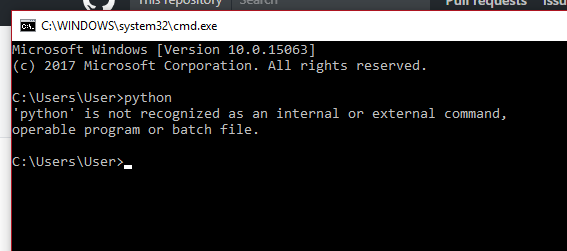
\includegraphics[width=1\textwidth]{Plagiarisme/cmd.PNG}}
	\caption{Contoh skirpt pada command prompt.}
	\label{cmd}
	\end{figure}
Pada gambar \ref{cmd} memberitahukan bahwa pada komputer yang saya pakai sekarang ini belum ada atau belum terinstall python.
Ketika python belum terinstall maka sistem akan mendeteksi bahwa comand yang diberikan tidak cocok dengan yang ada disistem. 
Akan tetapi kalau sudah terinstall maka akan memunculkan nama python begitu pula versi python yang di install.
Python menyediakan dukungan yang kuat untuk integrasi dengan bahasa pemrograman lain dan alat-alat bantu lainnya. 
Python hadir dengan pustakapustaka standar yang dapat diperluas serta dapat dipelajari hanya dalam beberapa hari.
Sudah banyak programmer Python yang menyatakan bahwa mereka mendapatkan produktivitas yang lebih tinggi. 
Mereka juga merasakan bahwa Python meningkatkan kualitas 

\subsection{Memasang Phyton}
Distribusi Python tersedia untuk berbagai macam platform. Anda hanya perlu mendownload kode biner yang berlaku untuk platform 
Anda dan menginstal Python.
Jika kode biner untuk platform Anda tidak tersedia, Anda memerlukan kompiler C untuk mengkompilasi kode sumber secara manual. 
Kompilasi kode sumber menawarkan fleksibilitas lebih dalam hal pilihan fitur yang Anda butuhkan dalam instalasi Anda.
Berikut adalah ikhtisar singkat tentang menginstal Python di berbagai platform :

\subsection{Menyiapkan PATH}
Program dan file eksekusi lainnya bisa berada di banyak direktori, 
jadi sistem operasi menyediakan jalur pencarian yang mencantumkan direktori yang dicari OS untuk executable.
Path disimpan dalam variabel lingkungan, yang merupakan string bernama yang dikelola oleh sistem operasi. 
Variabel ini berisi informasi yang tersedia untuk perintah shell dan program lainnya.
The path variabel disebut sebagai PATH di Unix atau jalan pada Windows (Unix adalah kasus sensitif, Windows tidak).
Di Mac OS, installer menangani detail jalur. Untuk meminta juru bahasa Python dari direktori tertentu, 
Anda harus menambahkan direktori Python ke path Anda.

\subsection{installasi Python pada windows}
	\begin{enumerate}
	\item Unduh Python 2.7 di python.org.
	\item Jalankan file instalasi Python yang telah diunduh. Secara default Python akan terinstall di folder C:>Python27.
	\item Selanjutnya mengatur variable environment, buka Control Panel->System and Security->System.
	\item Klik Advanced system settings, Environment Variables.
	\item Pada System variables, pilih Path, klik Edit.
	\item Pada Variable value, tambahkan ;C:>Python27.
	\end{enumerate}
	
\subsubsection{Pengujian Python pada windows}
	\begin{enumerate}
	\item Cara pertama: ketik python untuk menjalankan Python Interpreter. 
	      Jika berhasil akan ditampilkan versi Python yang digunakan beserta interpreternya. 
	      Coba ketikkan print “hello world” untuk menampilkan teks hello world.
	\item Cara kedua: buat file hello.py, yang isinya print “hello world”, 
	      simpan di mana saja suka-suka kamu, misalnya di D:>python-code. Buka command prompt, Run -> cmd. 
	      Kemudian masuk ke folder D:>python-code, lalu ketik python hello.py untuk menjalankan file Python yang telah dibuat.

\subsection{Installasi Python pada Unix/Linux}
	Berikutini adalah simple steps untuk menginstall python pada Unix/Linux.
	\begin{enumerate}
	\item Buka web browser dan ketik alamat https://www.python.org/downloads/
	\item Ikuti link untuk mendownload source code yang bisa digunakan oleh Unix/Linux
	\item Download dan kemudian extrak file
	\item Edit modules/setup file jika mau customize beberapa pengaturan
	\item Jalankan perintah ./configure script
	\item Installasi 
	\end{enumerate}
Lokasi standar penginstallan python ada pada /usr/local/bin dan libraries nya berada 
/usr/local/lib/pythonXX dimana XX adalah versi python yang di install.

\subsection{Setting Path pada Unix/Linux}
Untuk menambahkan direktori python di path pada Unix
\begin{enumerate}
\item In the csh shell – ketik setenv PATH $PATH:/usr/local/bin/python lalu tekan enter
\item In the bash shell(Linux) – ketik export ATH=$PATH:/usr/local/bin/python lalu tekan enter
\item In the sh or ksh shell – ketik PATH=$PATH:/usr/local/bin/python lalu tekan enter
\item Note - /usr/local/bin/python adalah path untuk direktori Python
\end{enumerate}

\subsection{Fitur Python}
Fitur-Fitur Python Python memiliki beberapa fitur yang menjadikan bahasa pemrograman ini berbeda dari bahasa lain antara lain :
\begin{enumerate}
\item Memiliki kepustakaan yang luas, dalam distribusi Python telah disediakan modul- modul siap pakai untuk berbagai keperluan.
\item Memiliki tata bahasa yang jernih dan mudah dipelajari.
\item Memiliki aturan layout kode sumber yang memudahkan
\item pengecekan, pembacaan kembali dan penulisan ulang kode sumber.
\item Berorientasi obyek.
\item Memiliki sistem pengelolaan memori otomatis (garbage collection, seperti java) Modular, mudah dikembangkan dengan menciptakan modul-modul baru; modul- modul tersebut dapat dibangun dengan bahasa Python maupun C/C++.
\item Memiliki fasilitas pengumpulan sampah otomatis, seperti halnya pada bahasa pemrograman Java, python memiliki fasilitas pengaturan penggunaan memory komputer sehingga para pemrogram tidak perlu melakukan pengaturan memory komputer secara langsung.
\item Memiliki banyak faslitas pendukung sehingga mudah dalam pengoprasiannya.
\end{enumerate}

\subsection{Pengujian}
Cara pertama: ketik python untuk menjalankan Python Interpreter. Jika berhasil akan ditampilkan versi Python yang digunakan beserta interpreternya. Coba ketikkan print “hello world” untuk menampilkan teks hello world.

C:>python
Python 2.7.11 (v2.7.11:6d1b6a68f775, Dec  5 2015, 20:40:30) [MSC v.1500 64 bit (AMD64)] on win32
Type "help", "copyright", "credits" or "license" for more information.
>>> print "hello world"
hello world
>>>

Cara kedua: buat file hello.py, yang isinya print “hello world”, simpan di mana saja suka-suka kamu, misalnya di D:\python-code. Buka command prompt, Run -> cmd. Kemudian masuk ke folder D:\python-code, lalu ketik python hello.py untuk menjalankan file Python yang telah dibuat.

D:\python-code>python hello.py
hello world


\subsection{Alasan Menggunakan Phyton}

Python memiliki konsep desain yang bagus dan sederhana, yang berfokus pada kemudahan dalam penggunaan. Kode Python dirancang untuk mudah dibaca, dipelajari, digunakan ulang, dan dirawat. Selain itu, Python juga mendukung pemograman berorientasi objek dan pemograman fungsional.
Python dapat meningkatkan produktivias dan menghemat waktu bagi para programmer. Untuk memperoleh hasil program yang sama, kode Python juga jauh lebih sedikit dibandngkan dengan kode yang ditulis menggunakan bahasa-bahasa pemograman lain seperti C, C++,C# maupun Java.


\subsection{Tipe Data Phyton}
	Menggunakan tipe Number

Tipe data Number digunakan untuk menyimpan nilai-nilai numerik. Tipe ini merupakan tipe data immutable, yang artinya jika kita mengubah nilai dari sebuah data, maka kita akan mengalokasikan obyek baru. Sama seperti tipe data lainnya, obyek Number dibuat ketika kita memberikan sebuah nilai padanya. Contoh:

>>>data = 1

Kita juga dapat mengubah nilai yang ada dalam variable data tersebut.

>>>data = data + 1
>>>data=3.50
>>>floatdat = 7.5
>>>data = floatdat

Kita dapat menghapus sebuah obyek ataupun banyak obyek dengan menggunakan pernyataan del. Misalnya:

>>>del data
>>>del data, floatdat

Python mengelompokkan tipe Number dalam 4 macam, yaitu:

Plain Integer
Plain integer atau bilangan bulat merupakan tipe data yang sering kita temui pada semua bahasa pemrograman. Integer ini mempunyai range nilai antara -2^32 sampai 2^31 – 1. Tipe ini juga dapat ditulis dalam bentuk octal (di tanda awalan “0”) maupun hexadesimal (ditandai awalan “0x” atau “0X”). Contoh:
10 100 6542 -784
083 -042 -0x43 0X61

Long Integer
Long integer sangat membantu kita untuk perhitungan di luar range nilai integer. Secara virtual, tidak ada batasan nilai tergantung besar virtual memory yang kita gunakan. Akhiran ‘l‘ atau ‘L‘ disetiap nilai bilangan bulat menandakan bahwa data tersebut bertipe long integer.
562718819L -0x526718L 012L -567299101L

Floating Point Real Number
Tipe ini sering disebut sebagai tipe real (atau float). Tipe ini sama dengan tipe double di C. Nilai float mempunyai dua bagian, bagian titik desimal dan bagian eksponensial. Tanda positif atau negatif diantara “e” merupakan tanda eksponen. Contoh nilai float:
0.0 14.5 -15.4 32.3+e18
-90.76712 -90. -32.54e100 70.2-E12

Complex Number
Sebuah bilangan kompleks biasanya ditunjukkan oleh bentuk a + bj, dimana a adalah bagian real dan b adalah bagian imajiner. Bagian imajiner merupakan bilangan di awal tanda “j” atau “J“. Berikut ini contoh bilangan kompleks:
3.14j 45j 54.56+12.1J 3e+36J

Bagian real dan imajiner dari bilangan kompleks dapat kita pisahkan menggunakan data atribut, yaitu menggunakan real dan imag. Sedangkan untuk mendapatkan konjugasi dari bilangan kompleks tersebut, kita dapat menggunakan metode conjugate().

>>> kompleks = 23.45-1.23J
>>> kompleks.real
23.45
>>> kompleks.imag
-1.23
>>> kompleks.conjugate()
(23.45+1.23j)

String merupakan salah satu tipe data yang sering digunakan dalam pemrograman Python. Sebuah string dapat dinyatakan sebagai kumpulan karakter yang dibatasi oleh satu atau dua tanda petik. Inilah contohnya,

>>> nama = "Klinik Python Indonesia"
>>> nama
'Klinik Python Indonesia'
>>> slm = 'Salam Python Dahsyat!'
>>> slm
'Salam Python Dahsyat!'
>>> print slm
Salam Python Dahsyat!

Dari contoh di atas, ketika kita memanggil variabel secara langsung maka akan ditampilkan isi dari variabel tersebut dengan sebuah tanda petik. Namun jika kita menggunakan pernyataan print, maka tanda petik tersebut akan dihilangkan.

Menampilkan Tanda Petik Sebagai String

Di dalam sebuah string tidak dapat berisi tanda petik yang sama dengan tanda petik yang digunakan oleh string tersebut. Misalkan, ketika kita menuliskan 'Py'thon' maka akan muncul pesan kesalahan (syntax error). Agar tidak muncul pesan kesalahan, kita bisa mengganti tanda petik luarnya dengan tanda petik ganda, misalnya "Py'thon". Tanda petik juga dapat ditulis setelah tanda backslash (\) agar dapat ditampilkan sebagai string.

>>> str = "Py'thon"
>>> str
"Py'thon"
>>> str2 = 'Py"thon'
>>> str2
'Py"thon'
>>> "\"OK, \" sampai ketemu lagi."
'"OK, " sampai ketemu lagi.'

Kode \n atau Triple Quotes Juga Boleh!

Jika kita ingin menuliskan string yang panjang dalam beberapa baris, maka kita perlu menambahkan tanda backslash diikuti huruf n (\n) sebagai tanda baris baru.

>>> teks = "Python adalah bahasa pemrograman yang powerfull.\nTerbukti Python bisa dijalankan di segala platform OS.\nJadi, saatnya kita menggunakan Python sebagai bahasa permrograman \nsehari-hari. Salam Python Dahsyat!"

Tanda \n akan memberikan perintah membuat baris baru jika kita memanggil teks dengan pernyataan print.

>>> print teks
Python adalah bahasa pemrograman yang powerfull.
Terbukti Python bisa dijalankan di segala platform OS.
Jadi, saatnya kita menggunakan Python sebagai bahasa permrograman
sehari-hari. Salam Python Dahsyat!

Kita juga dapat menggunakan tanda petik tiga (triple quotes), """ atau ''', untuk menuliskan sebuah string yang panjang dalam beberapa baris.

>>> teks = """Python adalah bahasa pemrograman yang powerfull.
... Terbukti Python bisa dijalankan di segala platform OS.
... Jadi, saatnya kita menggunakan Python sebagai bahasa pemrograman
... sehari-hari. Salam Python Dahsyat!"""

Tampilan teks dengan pernyataan print seperti di bawah ini,

>>> print teks
Python adalah bahasa pemrograman yang powerfull.
Terbukti Python bisa dijalankan di segala platform OS.
Jadi, saatnya kita menggunakan Python sebagai bahasa pemrograman
sehari-hari. Salam Python Dahsyat!

Menggabungkan String

Untuk menggabungkan dua buah string atau lebih, kita dapat menggunakan operator +. Sedangkan untuk menggandakan string, kita gunakan operator *.

>>> blog = 'Klinik' + 'Python'
>>> blog
'KlinikPython'
>>> newblog = blog*5
>>> newblog
'KlinikPythonKlinikPythonKlinikPythonKlinikPythonKlinikPython'
>>> blog *= 4
>>> print blog
KlinikPythonKlinikPythonKlinikPythonKlinikPython

Jika dua string ditulis secara berurutan, maka secara langsung kedua string tersebut akan digabungkan.

>>> blog = 'Klinik''Python'
>>> blog
'KlinikPython'

Menentukan Panjang String

Panjang dari sebuah string dapat kita temukan dengan menggunakan fungsi len().

>>> len(blog)
12

Memecah String

Tidak seperti bahasa lainnya, Python tidak mendukung tipe Karakter. Untuk mengambil satu karakter atau lebih dari sebuah string, kita dapat memecah string tersebut menggunakan indeks (disebut Metode Irisan). Irisan terdiri dari dua indeks yang dipisahkan tanda koma.

>>> buah = 'Nanas'
>>> buah[0]
'N'
>>> buah[0:2]
'Na'
>>> buah[0:4]
'Nana'
>>> buah[0:5]
'Nanas'

Dari contoh di atas, panjang string buah adalah 5. Ketika kita menghitung maju, indeks bernilai 0 sampai (panjang-string – 1) dimulai dari kiri ke kanan. Maka dari itu, kita dapat mengakses setiap karakter dalam range 0 sampai 4.

Sebuah string juga dapat dihitung mundur, dengan indeks -1 sampai (negatif panjang-string) dimulai dari kanan ke kiri. Berikut gambaran lengkapnya, baik itu penghitungan maju atau mundur.

Contoh penggunaan penghitungan mundur,

>>> buah[-1]
‘s’
>>> buah[-5]
‘N’
>>> buah[-5:-1]
‘Nana’
>>> buah[1:-1]
‘ana’

Jika kita lupa berapa nilai indeks awala atau indeks akhir, kita dapat kosongkan indeks tersebut.

>>> buah[:3]
‘Nan’
>>> buah[2:]
‘nas’

Pengosongan indeks akan menyebabkan semua string ditampilkan.

>>> buah[:]
‘Nanas’

String Bersifat Immutable

Tipe data String pada Python bersifat immutable, yang artinya sekali dibuat maka tidak dapat diubah kembali. Ada pertanyaan bagus, jika string bersifat immutable, mengapa kita bisa mengubah nilai dari variabel string tersebut? Jawabannya sangat sederhana. Ketika kita memberikan nilai yang berbeda pada variabel string, sebuah obyek baru berhasil kita buat. Lihat contoh berikut,

>>> nama = "Klinik"
>>> nama
'Klinik'
>>> id(nama)
3076962016L
>>> nama = "Python"
>>> id(nama)
3077289888L

Catat bahwa ketika string nama telah kita buat, maka identitas dari variabel ini dapat kita ketahui dengan menggunakan fungsi id(). Jika kita ubah nilai dari variabel nama tersebut, maka identitasnya juga berubah. Hal ini menandakan bahwa obyek baru telah dibuat. Penggantian nilai pada string pada posisi indeks tertentu akan menghasilkan pesan kesalahan.

>>> nama[0] = 'K'
Traceback (most recent call last):
File "", line 1, in
TypeError: 'str' object does not support item assignment

Kita juga dapat menambahkan sebuah string baru pada string lama.

>>> 'Si' + nama[0]
'SiP'
>>> 'J' + nama[1:]
'Jython'

